% Modified for use with Wiley Interdisciplinary Reviews Copyright (C) (2016). All rights reserved.
\documentclass[12pt]{article}

\setlength{\oddsidemargin}{0in}  %left margin position, reference is one inch
\setlength{\textwidth}{6.5in}    %width of text=8.5-1in-1in for margin
\setlength{\topmargin}{-0.5in}    %reference is at 1.5in, -.5in gives a start of about 1in from top
\setlength{\textheight}{9in}     %length of text=11in-1in-1in (top and bot. marg.) 

\usepackage{amsmath,amssymb,amsthm,mycommands1}
\usepackage[round]{natbib}
\usepackage{graphicx}% Include figure files
\usepackage{caption}
\usepackage{color}% Include colors for document elements
\usepackage{dcolumn}% Align table columns on decimal point
\usepackage{bm}% bold math
\usepackage{float}
\usepackage{hyperref} % hyperref must be loaded before apacite
%\usepackage{apacite}
%\bibliographystyle{apacite}
\hypersetup{ colorlinks = true, citecolor = blue, urlcolor = blue}
%\usepackage[nolists, nomarkers, figuresfirst]{endfloat}

%% For pstricks
\usepackage[pdf]{pstricks}
\usepackage{epsfig}
\usepackage{pst-grad} % For gradients
\usepackage{pst-plot} % For axes
\usepackage[space]{grffile} % For spaces in paths
\usepackage{etoolbox} % For spaces in paths
\makeatletter % For spaces in paths
\patchcmd\Gread@eps{\@inputcheck#1 }{\@inputcheck"#1"\relax}{}{}
\makeatother

\definecolor{background-color}{gray}{0.98}

\title{Robust Principal Component Analysis: a Review}
% The title should not exceed 20 words. Please be original and try to include keywords, especially before a colon if applicable, as they will increase the discoverability of your article. Visit http://media.wiley.com/assets/7158/18/SEO_For_Authors.pdf for tips on search engine optimization.

\author{Subhabrata Majumdar
\thanks{University of Florida Informatics Institute, 432 Newell Drive, CISE Bldg E251, Gainesville, FL 32611}, Snigdhansu Chatterjee
\thanks{School of Statistics, University of Minnesota, 313 Ford Hall, 224 Church St SE, Minneapolis, MN 55455}}
% The preferred (but optional) format for author names is First Name, Middle Initial, Last Name.
% Wiley requires that all authors disclose any potential conflicts of interest.  Any interest or relationship, financial or otherwise, that might be perceived as influencing an author’s objectivity is considered a potential conflict of interest. The existence of a conflict of interest does not preclude publication.

%\date{}

\DeclareMathOperator*{\ve}{vec}
\DeclareMathOperator*{\diag}{diag }
\DeclareMathOperator*{\Tr}{Tr}
\DeclareMathOperator*{\argmin}{arg\,min}
\DeclareMathOperator*{\argmax}{arg\,max}

\begin{document}
\maketitle

\newtheorem{Theorem}{Theorem}[section]
\newtheorem{Lemma}[Theorem]{Lemma}
\newtheorem{Corollary}[Theorem]{Corollary}
\newtheorem{Proposition}[Theorem]{Proposition}
\newtheorem{Conjecture}[Theorem]{Conjecture}
\theoremstyle{definition} \newtheorem{Definition}[Theorem]{Definition}

\date{}
%\author{Subhabrata Majumdar, Snigdhansu Chatterjee}
\maketitle

%{(\colrbf will change)} We introduce a composition of the spatial sign function \citep{LocantoreEtal99} with transformations on functions that are essentially the outlyingness maps of \cite{zuo00}, with a few restrictions for technical convenience. After a brief consideration of its performance in the location problem for elliptical distributions, we define a multivariate rank vector using this. We discuss several aspects of its performance in estimating components of the covariance matrix in the data-generating elliptical distribution: its eigenvectors, eigenvalues and the covariance matrix itself. Several simulation studies and data examples outline the utility of these methods, and we also discuss their implementation in Sufficient Dimension Reduction \citep{AdragniCook09} and functional outlier detection.
\vspace{.5cm}

\begin{center}
\subsubsection*{\small Article Type:}
Advanced Review
%The Article Type denotes the intended level of readership for your article. An Editor may have mentioned a specific Article Type in your invitation letter; if so, please let them know if you think a different Article Type better suits your topic.

\hfill \break
\thanks

\subsubsection*{Abstract}
\begin{flushleft}
Principal Component Analysis (PCA) is widely used many scientific domains. Accurately estimating the underlying low-rank structure in a data matrix in presence of corrupted entries is a problem that has achieved considerable attention in statistical literature. In this paper we review techinques that deal with this robust estimation problem. These span statistical methods useful for accurate estimation of principal components in presence of outlying samples, as well as the recently proposed Principal Component Pursuit approach that is effective when the data matrix contains sparse noise. We summarize the research in these two domains, and present data examples for their comparative evaluation. Finally, we also review methods that perform robust versions of kernel PCA and functional PCA.
\end{flushleft}
\end{center}

\subsubsection*{Keywords}
Principal Component Analysis; Robustness; ROBPCA; Spatial signs; data depth; Principal Component Pursuit

\clearpage

\renewcommand{\baselinestretch}{1.5}
\normalsize

\clearpage

%
\section*{\sffamily \Large INTRODUCTION}

Principal component Analysis (PCA) is one of the oldest, yet most widely used methods of unsupervised multivariate analysis. For a data matrix $\bfX \in \BR^{n \times p}$ containing observations in $p$ variables for $n$ samples, each column having mean 0, principal components are defined as $p$-dimensional vectors $\bfw_k, 1 \leq k \leq p$ such that
%
\begin{align}\label{eqn:eqnPCA}
\bfw_1 &= \argmax_{\| \bfw \| = 1} \bfw^T \bfX^T \bfX \notag\\
\bfw_k &= \argmax_{\| \bfw \| = 1} \bfw^T \bfR_k^T \bfR_k \bfw; \quad \bfR_k = \bfX - \sum_{s=1}^{k-1} \bfX \bfw_s \bfw_s^T \quad \text{for } 1< k \leq p
\end{align}
%
Following a lagrange multiplier approach, the eigenvectors of $\bfX^T \bfX$, equivalently the right singular vectors obtained from the singular value decomposition of $\bfX$ provide solutions to (\ref{eqn:eqnPCA}).

{\colrbf more stuff}

{\colrbf robustness towards outliers}

{\colrbf robustness towards corrupted entries}

{\colrbf combine?}
\section{Robust covariance estimation, data transformation, and beyond}
\label{Section:sec2}

\subsection{Robust covariance matrices, projection pursuit}

The earliest approaches to robust PCA were based on robustly estimating the population covariance matrix, and using eigenvectors of that estimate as principal components. Some methods of robust covariance matrix estimation include the Minimum Volume Ellipsoid estimator \citep{Rousseeuw84}, a projection-based estimator by \citep{maronna76}, the Minimum Covariance Determinant (MCD) estimator \citep{rousseeuw85} and the Stael-Donoho estimators \citep{MaronnaYohai95,ZuoCui05}. Although these estimators have high breakdown points, they suffered from two severe drawbacks. Firstly the explicit evaluation of the population covariance matrix meant that obtaining principal components were not possible when $n < p$. Secondly, even when $n > p$, these methods become computationally intensive with large data dimensions.

\cite{LiChen85} first introduced the idea of Projection Pursuit (PP) in robust PCA to alleviate these problems. Notice that the case for $k=1$ in (\ref{eqn:eqnPCA}) can be rewritten as
%
$$
\bfw_1 = \argmax_{\| \bfw \| = 1} Var (\bfX \bfw)
$$
%
The proposal of \cite{LiChen85} was to simply use a robust univariate scale estimator $s_n$ (e.g. median, MCD) to obtain the robust PCs from a size $n$ sample $\bfX = (\bfx_1, \ldots, \bfx_n)$:
%
\begin{align*}
\hat \bfw_1^\text{PP} &= \argmax_{\| \bfw \| = 1} s_n ( \bfw^T \bfx_1, \ldots, \bfw^T \bfx_n );\\
\hat \bfw_k^\text{PP} &= \argmax_{\| \bfw \| = 1; \bfw \perp \bfw_s, s < k} s_n ( \bfw^T \bfx_1, \ldots, \bfw^T \bfx_n ) \quad \text{for } 1< k \leq p
\end{align*}
%
Aside from not having any restrictions for high-dimensional data, the PP approach allowed the flexibility of using any robust univariate scale estimator, and sequential estimation of the principal components. PP-based robust PCA became a popular method for chemometric data analysis in the 1990-s and early 2000-s, mainly due to the algorithmic developments by \cite{XieEtal93}, \cite{HubertEtal02} and \cite{CrouxEtal07}.

The ROBPCA method of \cite{hubert05} combines the above two approaches. Specifically, ROBPCA consists of the following steps:
%
\begin{itemize}
\item Do an initial dimension reduction of the data matrix: $\bfX_{n \times p} \mapsto \bfZ_{n \times r}, r \leq p$ by projecting all data points on the subspace formed by the right singular vectors of $\bfX$:
%
$$
\bfX = \bfU_{n \times r} \bfD_{r \times r} \bfV_{r \times p}; \quad
\bfZ = \bfU \bfD
$$

\item Calculate the outlyingness of all samples:
%
$$
O(\bfz_i) = \max_{\bfv \in B} \frac{| \bfz_i^T \bfv - m_n (\bfz_j^T \bfv)|}{s_n (\bfz_j^T \bfv )}
$$
%
where $m_n$ and $s_n$ are robust location and scale estimators, respectively. When $\binom{n}{2} < 250$, $B$ is the set of vectors passing through all pairs of sample points, and is a collection of 250 randomly chosen non-zero vectors in $\BR^{r}$ otherwise.

Use the top $k$ PCs calculated from the $h$ least outlying points ($k \leq r; k, h$ suitably chosen) to transform the data again:
%
$$
\bfZ^* =  \bfZ \bfP_0; \quad \bfP_0 \in \BR_{r \times k}
$$

%\item If $s_n (\bfz_j^T \bfv ) = 0$ for some $\bfv$, then all samples are projected onto the hyperplane orthogonal to that $\bfv$ and these projection are taken as the new observations to work with. This optional step potentially reduces data dimension to some $r_1 \leq r_0$. for notational convenience, we still refer to this transformed data as $\bfZ$.

\item Robustly estimate the scatter matrix of $\bfZ^*$, take its eigenvectors as the estimated robust PCs.
\end{itemize}

As \cite{hubert05} showed through application on simulated and real data, the combination of a PP approach (first step) and robust scatter matrix estimation (third step) used by ROBPCA results in efficiency gains in estimating population principal components, as well as better detection of outlying points, compared to either of the previous types of methods for robust PCA.

\subsection{Data transformation and $M$-estimation}

A parallel approach towards robust PCA has also been developed by researchers, that is focused on the usage of robust transformations on the data, specifically multivariate signs and ranks, and related $M$-estimates of scatter. First introduced by \cite{MottonenOja95}, the multivariate sign or \textit{spatial sign} of a vector $\bfx \in \BR^p$ with respect to a location parameter $\bfmu \in \BR^p$ is defined as:
%
$$
\bfS (\bfx) = \frac{\bfx  - \bfmu }{\| \bfx - \bfmu\|} \BI_{\bfx \neq \bfmu}
$$
%
When $\bfx$ is a random sample from an elliptical distribution, the sign transformation keeps the population eigenvectors constant. Since all vectors in the same direction get mapped to the same spatial sign regardless of their magnitude, eigenvector estimates calculated from the Sign Covariance Matrix (SCM), or equivalently the SVD of a sign transformed data matrix can act as robust PCs \citep{LocantoreEtal99,visuri00}.

\begin{figure}[t]
\centering
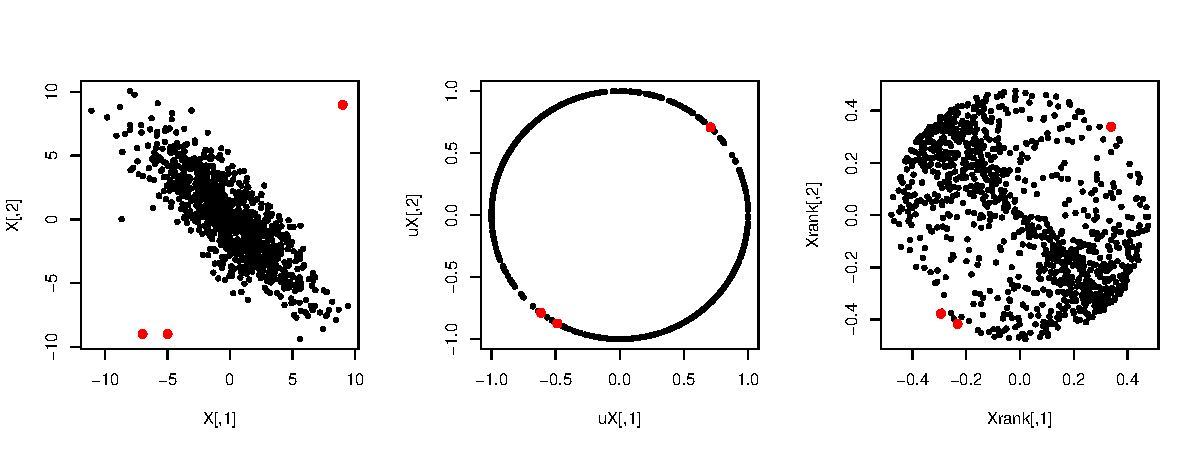
\includegraphics[width=\textwidth]{allthree}
\caption{allthree}
\label{fig1:allthree}
\end{figure}

There are two components of a multivariate data point: its direction and magnitude. Spatial sign discards the magnitude and only uses the direction. Consequently, although the sign transformation provides an intuitively simple way of robustly estimating population eigenvectors, the estimates are not very accurate, in terms of asymptotic and finite-sample efficiencies \citep{Majumdar15}. In fact, \cite{magyar14} showed that the eigenvectors of the $M$-estimate of scatter proposed by \cite{tyler87} has uniformly lower asymptotic risk than those obtained from the SCM.

\cite{Majumdar15} rectified this by weighting the spatial signs by a bounded distance measure from the origin. They used data depth \citep{zuo00} to construct these weight functions. For some $\bfy \in \BR^p$ and a set of points in $\BR^p$, say $(\bfy_1, \ldots, \bfy_n)^T = \bfY$, data depth (denoted by $D(\bfy, \bfY)$) provides an affine invariant scalar measure of how close $\bfy$ is to the data cloud. The depth-based weighted spatial signs\cite{Majumdar15} are explicitly constructed as:
%
\begin{align}
\tilde \bfx = \left[ \sup_{\bfz} D(\bfz, \bfX) - D(\bfx, \bfX) \right] \bfS( \bfx - \bar \bfX )
\end{align}
%
The transformation $\bfx \mapsto \tilde \bfx$ preserves the magnitude information of the point: points with the same direction but different magnitudes get mapped further from the origin as the magnitude increases. However, due to the boundedness of data depth, this mapping limits the maximum distance an outlying point can get mapped to (see figure \ref{fig1:allthree}). Thus the weighted sign transformation improves upon the sign-based PCA in terms of lower estimation errors for elliptic underlying distributions, while still preserving robustness properties like high breakdown points and bounded influence functions \citep{Majumdar15}.

\subsection{Robust PCA and outlier detection}
Aside from obtaining a lower dimensional projection of the data matrix $\bfX$ in spite of outliers that is close enough to the projection of $\bfX$ by the first few population eigenvectors, detecting the outliers themselves is also closely associated with robust PCA. These samples can be of interest for mechanistic reasons. For example in the analysis of near infra-red absorbance for 39 gasoline samples over 226 wavelengths using ROBPCA \citep{hubert05}, six compounds are flagged as outliers, and these turn out to be the only samples containing alcohol. \cite{hubert05} also introduced a notion of outlier diagnostics that is applicable to any method of robust PCA and can serve as a means to compare different relevant techniques as well.

We illustrate this in \ref{fig:figROBPCA}. Here we consider data in 3 dimensions, and consider the relative position of the samples with respect to the two-dimensional principal component subspace $\cM$. We can classify such points into four categories:

\begin{enumerate}
\item{\it Regular observations}: points that form a homogeneous group close to $\cM$ ($A$ and $B$ in figure);
\item{\it Good leverage points}: points that lie close to $\cM$, but at a distance from the regular observations ($C$ in figure);
\item{\it Orthogonal outliers}: These points (point $D$ in figure) lie far away from their projections on $\cM$ (point $D'$, but the projections themselves are close to the regular observations;
\item{\it Bad leverage points}: These points are also far away from their projections on $\cM$ ($E$ and $E'$ respectively), but the projections are also far away from the regular observations.
\end{enumerate}

\cite{hubert05} introduced the concept of \textit{score distance} (SD) and \textit{orthogonal distance} (OD) to distinguish between these four types of points. With our notation, for the $i^\text{th}$ observation these distances are defined as:
%
$$
SD_i = \sum_{j=1}^q \frac{t_{ij}}{\lambda_j};\
\quad OD_i  =\| ( \bfI - \bfW_k \bfW_k^T) (\bfx_i - \bfmu) \|
$$
%
The SD can be interpreted as the weighted distance of the projection of a point on the hyperplane formed by the first $k$ PCs, while OD is the orthogonal distance of that point and the $k$-PC hyperplane. It is now clear from our picture that regular observations have low values of both SD and OD, while bad leverage points have high values of both. An orthogonal outlier has small SD but large OD, whereas a good leverage point has high SD but small OD. To explicitly classify sample points into these 4 categories, \cite{hubert05} use $\sqrt {\chi^2_{k,0.975}}$ and $[ \hat \mu (OD^{2/3}) + \hat \sigma (OD^{2/3}) \Phi^{-1} (0.975) ]^{3/2}$ as upper cutoffs for score distance and orthogonal distance, respectively. Here $\hat \mu$ and $\hat \sigma$ are univariate MCD estimators, and $\Phi$ is the standard normal cumulative distribution function.
\section*{\sffamily \Large PRINCIPAL COMPONENT PURSUIT}
\label{section:sec3}

The above notion of outliers depends on the fact that the $n \times p$ data matrix $\bfX$ is composed of observations from several independent samples in its rows, and some of these samples have corrupted observations. However, in many practical situations, rows of $\bfX$ might not be independent, the corrupted observations can have a pattern across samples, or both. For example in face or handwriting recognition, each individual picture can be taken as a data matrix. The value of a pixel takes corresponds to an entry in the data matrix, with noisy pixels denoting corrupted measurements. Although the underlying low-rank structure is still of interest in such situations, for example the face of a person or a handwritten digit, this problem is fundamentally different because of the inherent structure present in the data.

\cite{CandesEtal09} first introduced {\it Principal Component Pursuit} (PCP), which decomposes the data matrix into low-rank and sparse components to tackle the above situation. Formally, PCP considers the following additive model:
%
\begin{align}\label{eqn:PCPmodel}
\bfX = \bfL_0 + \bfS_0
\end{align}
%
with rank$(\bfL_0) = r < p$ and $\bfS_0$ sparse. The low-rank and sparse structures are recovered using nuclear norm penalization on the first component and $\ell_1$-norm penalization on the second component, respectively:
%
\begin{align}\label{eqn:PCPobj}
& \text{minimize } \| \bfL \|_* + \lambda \| \bfS \|_1; \quad \text{subject to } \bfL + \bfS = \bfX
\end{align}
%
where $\|.\|_*$ denotes the nuclear norm of a matrix, i.e. sum of its singular values, and $\|.\|_1$ denotes $\ell_1$-norm, i.e. sum of the absolute values of its entries, and $\lambda $ is a tuning parameter that determines the amount of sparsity permitted in $\bfS$. \cite{CandesEtal09} proved that given the true underlying structure is indeed low-rank-plus-sparse, i.e. adheres to the decomposition in (\ref{eqn:PCPmodel}), a polynomial time algorithm based on convex programming can exactly recover these matrices, and this is possible for arbitrary magnitudes of entries in the sparse component.

\subsection*{\sffamily \large PCP and matrix completion}
Both the polynomial time algorithm and arbitrary magnitude of corrupted entries are strengths of PCP over traditional methods of robust PCA. Another reason the PCP is attractive by itself is because with slight modifications, it can perform robust matrix completion. The matrix completion problem attempts to fill in a data matrix $\bfY$ through nuclear norm minimization when only a subset $\Omega \subset \{ 1, \ldots, n\} \times \{ 1, \ldots, p\}$ of its entries are observed. Formally stated, the problem amounts to
%
$$
\text{minimize } \| \bfL \|_*; \quad \text{ subject to } \bfP_\Omega \bfL = \bfY
$$
%
where $\bfP_\Omega$ is the known indicator matrix of non-missing entries: $(\bfP_\Omega)_{ij} = \BI_{(i,j) \in \Omega}$. PCP simply assumes there is a sparse noise component in the incomplete data: $\bfY = \bfP_\Omega (\bfL_0 + \bfS_0)$, and recovers the low-rank structure:
%
\begin{align}\label{eqn:PCPMCobj}
& \text{minimize } \| \bfL \|_* + \lambda \| \bfS \|_1; \quad \text{subject to } \bfP_\Omega(\bfL + \bfS) = \bfY
\end{align}
%

\cite{CandesEtal09} showed that it is possible to solve this problem with minimal modifications to their original PCP algorithm that solves (\ref{eqn:PCPobj}). Multiple further studies provided improvements for several aspects of this basic setup. The work of \cite{ChenEtal11} is prominent among them. In particular, they assumed the presence of both errors and missing entries, with deterministic or random support for each of them, and provided theoretical performance guarantees when the fraction of observed entries vanishes as $n \rightarrow \infty$. They also performed worst-case analysis for the errors-only or missing-only scenarios.

\subsection*{\sffamily \large Modifications}
In a subsequent paper, \cite{ZhouEtal10} added an entrywise noise component $\bfZ$ to the objective functions in (\ref{eqn:PCPobj}):
%
\begin{align}\label{eqn:PCPobjZ}
& \text{minimize } \| \bfL \|_* + \lambda \| \bfS \|_1; \quad \text{subject to } \bfL + \bfZ + \bfS = \bfX
\end{align}
%
and (\ref{eqn:PCPMCobj}):
%
\begin{align}\label{eqn:PCPMCobjZ}
& \text{minimize } \| \bfL \|_* + \lambda \| \bfS \|_1; \quad \text{subject to } \bfP_\Omega(\bfL + \bfZ + \bfS) = \bfY
\end{align}
%
This brought the PCP formulation closer to the classical robust PCA setup that separates a lower-dimensional component in presence of both data-wide additional noise and corrupted entries, with the advantage that here the magnitude and structure of corrupted entries can be arbitrary. Further modifications of PCP include the case when the lower-dimensional component is a union of multiple lower dimensional subspaces \citep{WohlbergEtal12}, adding an $\ell_1/\ell_2$-penalization term on $\bfL$ \citep{TangNehorai11}, a dual formulation of the problem \citep{BeckerEtal11}, and non-convex robust matrix completion \citep{ShangEtal14}. PCP has been an active area of research in the signal and image processing community for the past few years. Further details on modifications of the PCP, algorithmic developments, and its applications in video surveillance can be found in \cite{Bouwmans14}.
\section*{\sffamily \Large NUMERICAL EXAMPLES}
\label{section:sec4}

We now present in detail the two data analytical scenarios to demonstrate the comparative performance and applicability of the different approaches of robust PCA discussed until now.

\subsection*{\sffamily \large Bus data}
Following the analysis in \cite{maronna06}, pp. 213, we set aside variable 9 and scale the other variables by dividing with their respective median absolute deviations (MAD). We do this done because all the variables had much larger standard deviations compared to their MADs, and variable 9 had MAD = 0. Following this, we compare the performances of the classical PCA (CPCA), PCA based on the eigenvector estimate from the MCD covariance matrix (MPCA), spatial sign-based PCA (SPCA), depth-based weighted sign PCA (DPCA), ROBPCA, and PCP.
We use projection depth as our choice of depth function while doing DPCA.

For all classical PCA methods, we set the number of PCs at 3. We compare the above methods using the distance of actual data and their projections on the principal component space. For PCP, these are is simply row norms of the sparse matrix $\bfS_0$ obtained from the procedure, while for other methods this is the orthogonal distances of corresponding samples. Each of its column lists different quantiles of the squared orthogonal distance for a sample point from the hyperplane formed by top 3 PCs estimated by the corresponding method. Table \ref{table:bus_table2} presents the different quantiles of squares of these distances for all the methods. For DPCA, the estimated principal component subspaces are closer to the data than CPCA for more than 90\% of samples, and the distance only becomes larger for higher quantiles. This means that for CPCA, estimated basis vectors of the hyperspace get pulled by extreme outlying points, while the influence of these outliers is very low for DPCA. SPCA and ROBPCA perform very closely in this respect, the percentage of points that have less squared distance than CPCA being between 80\% and 90\% for both of them. This percentage is only 60\% for PCP and 50\% for MPCA, which suggests that the corresponding 3-dimensional subspace estimated by MCD is possibly not an accurate representation of the truth, and there is probably enough noise in the data apart from the low-rank and sparse components estimated by PCP.

%\begin{table}[t]
%\centering
%    \begin{tabular}{c|ccccc}
%    \hline
%    \begin{large} $q$ \end{large} & \multicolumn{5}{c}{Method of PCA}         \\ \cline{2-6}
%    ~                   & CPCA     & SPCA & ROBPCA & MPCA & DPCA \\\hline 
%    1                   & 0.188         & 0.549     & 0.410  & 0.514     & 0.662     \\
%    2                   & 0.084         & 0.272     & 0.214  & 0.337     & 0.359     \\
%    3                   & 0.044         & 0.182     & 0.121  & 0.227     & 0.237     \\
%    4                   & 0.026         & 0.135     & 0.083  & 0.154     & 0.173     \\
%    5                   & 0.018         & 0.099     & 0.054  & 0.098     & 0.115     \\
%    6                   & 0.012         & 0.069     & 0.036  & 0.070     & 0.084     \\ \hline
%    \end{tabular}
%    \caption{Unexplained proportions of variability by PCA models with $q$ components for bus data}
%    \label{table:bus_table1}
%\end{table}

\begin{table}[t]
\centering
    \begin{tabular}{c|cccccc}
    \hline
    Quantile & \multicolumn{6}{c}{Method of PCA}         \\ \cline{2-7}
    ~                   & CPCA     & SPCA & ROBPCA & MPCA & DPCA & PCP\\\hline 
    10\%      & 1.9       & 1.2       & 1.2    & 1.0       & 1.2       & 1.3\\
    20\%      & 2.3       & 1.6       & 1.6    & 1.3       & 1.6       & 1.8\\
    30\%      & 2.8       & 1.8       & 1.8    & 1.7       & 1.9       & 2.1\\
    40\%      & 3.2       & 2.2       & 2.1    & 2.1       & 2.3       & 2.5\\
    50\%      & 3.7       & 2.6       & 2.5    & 3.1       & 2.6       & 3.2\\
    60\%      & 4.4       & 3.1       & 3.0    & 5.9       & 3.2       & 3.8\\
    70\%      & 5.4       & 3.8       & 3.9    & 25.1      & 3.9       & 5.7\\
    80\%      & 6.5       & 5.2       & 4.8    & 86.1      & 4.8       & 11.9\\
    90\%      & 8.2       & 9.0       & 10.9   & 298.2     & 6.9      & 80.2\\
    Max       & 24        & 1037      & 1055   & 1037      & 980      & 1157\\\hline
    \end{tabular}
    \caption{Quantiles of squared data-to-projection distances for bus data}
    \label{table:bus_table2}
\end{table}

\subsection*{\sffamily \large Image denoising}
As mentioned before, a major area of application of robust PCA, and PCA in general, is to extract the underlying low-rank structure in image recognition problems that are often high-dimensional in nature. Although PCP was designed keeping this very generative model (i.e. (\ref{eqn:PCPmodel})) in mind, \cite{ZhaoEtal14} showed that even the classical PCA performs fairly well in comparison of low-rank-plus-sparse methods to remove certain types of noise from an image, as well as background subtraction of videos.

\begin{figure}[t]
\centering
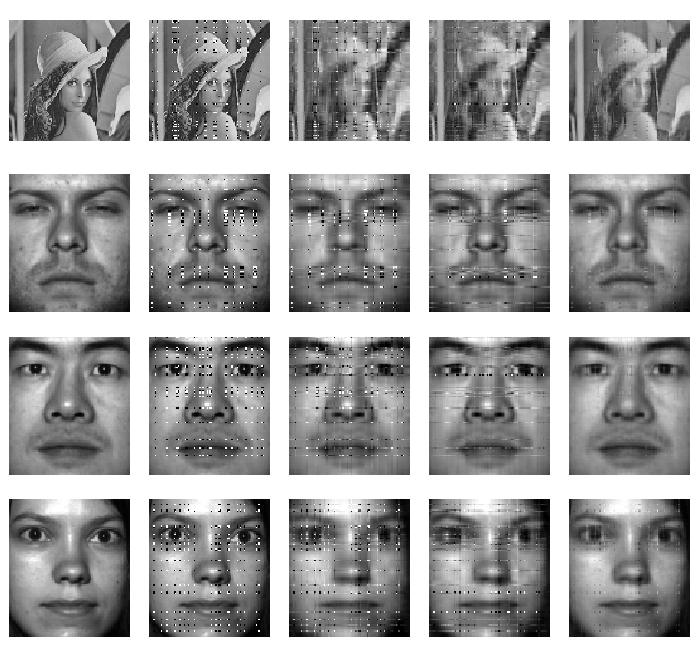
\includegraphics[width=.8\textwidth]{all_denoise}
\caption{Denoising results of four images. Left to right in a row indicates the original image, image with noise added, and denoising by DPCA, ROBPCA and PCP, respectively.}
\label{fig:figDenoise}
\end{figure}

We first resize our images: the lenna image from $128 \times 128$ to $96 \times 96$ and the Yale images from $192 \times 168$ to $96 \times 84$. After this we randomly select 10\% of the pixels from each image and turn their values to 0 or 1 with probability 0.5. Such noise occurs naturally in image recognition problems, and degrades image quality as well as the performance of image classification algorithms \citep{Qiuetal04}. Following this we center and scale each of these matrices of pixel values and apply DPCA, ROBPCA and PCP on them. We take the top 10 estimated PCs for DPCA and ROBPCA to reconstruct the images. Figure~\ref{fig:figDenoise} gives the results obtained from each of these methods. The first and second images in each row denote the original image with and without speckle noise, while the others give denoised versions from the three methods. PCP has the best performance: it recovers the faces almost perfectly, and does better than the other two methods for the Lenna image. The structure in the data seem to have affected the performance of DPCA and ROBPCA, which retain some of the noise in the reconstructed versions. Using a larger number of PCs retains the noises as well. Finally, the performance of all methods suffer when they are applied on the Lenna image, which is a relatively complex image.
\section*{\sffamily \Large ROBUST PCA IN OTHER SPACES}
\label{section:Others}

\subsection*{\sffamily \large Kernel PCA}

\subsection*{\sffamily \large Functional PCA}
\section{Conclusion}



\bibliographystyle{apalike}
\bibliography{reviewbib}

\end{document}